%%%%%%%%%%%%%%%%%%%%%%%%%%%%%%%%%%%%%%%%%%%%%%%%%%%%%%%%%%%
% --------------------------------------------------------
% Tau
% LaTeX Template
% Version 2.4.4 (28/02/2025)
%
% Author: 
% Guillermo Jimenez (memo.notess1@gmail.com)
% 
% License:
% Creative Commons CC BY 4.0
% --------------------------------------------------------
%%%%%%%%%%%%%%%%%%%%%%%%%%%%%%%%%%%%%%%%%%%%%%%%%%%%%%%%%%%

\documentclass[9pt,a4paper,column,twoside]{tau-class/tau}
\usepackage[english]{babel}

%% Spanish babel recomendation
% \usepackage[spanish,es-nodecimaldot,es-noindentfirst]{babel} 

%% Draft watermark
% \usepackage{draftwatermark}

%----------------------------------------------------------
% TITLE
%----------------------------------------------------------

\journalname{Intro Microelectronic Circuits with Laboratory}
\title{Resistors and Bipolar Transistors}

%----------------------------------------------------------
% AUTHORS, AFFILIATIONS AND PROFESSOR
%----------------------------------------------------------

\author[1]{Anika Mahesh}
\author[1]{Elias Tuthill}
\author[1]{Henry Tejada Deras}

%----------------------------------------------------------

\affil[1]{Franklin W. Olin College of Engineering}

%----------------------------------------------------------
% FOOTER INFORMATION
%----------------------------------------------------------

\institution{Franklin W. Olin College of Engineering}
\footinfo{Intro Microelectronic Circuits with Laboratory}
\theday{TBD}
\leadauthor{Mahesh et. al.}

%----------------------------------------------------------

\begin{document}
		
    \maketitle 
    \thispagestyle{firststyle} 
    % \tauabstract 
    % \tableofcontents
    % \linenumbers 
    
%----------------------------------------------------------
% 2 - 1k 10k 100k
% 3 - 1k
% 4 - 1k (emitter and GND), 10k, 5k, 2k (5V and collecter)
\section{Bipolar Transistor Characteristics}
	\subsection{Results}
	\begin{figure}[H]
 		\centering
   		\includegraphics[width=0.6\linewidth]{../diagrams/lab3_c1.pdf}
   		\caption{The schematic for the experimental setups used in Experiment 1.}\label{fig:exp1_diag}
	\end{figure}
	\begin{figure}[H]
		\centering
		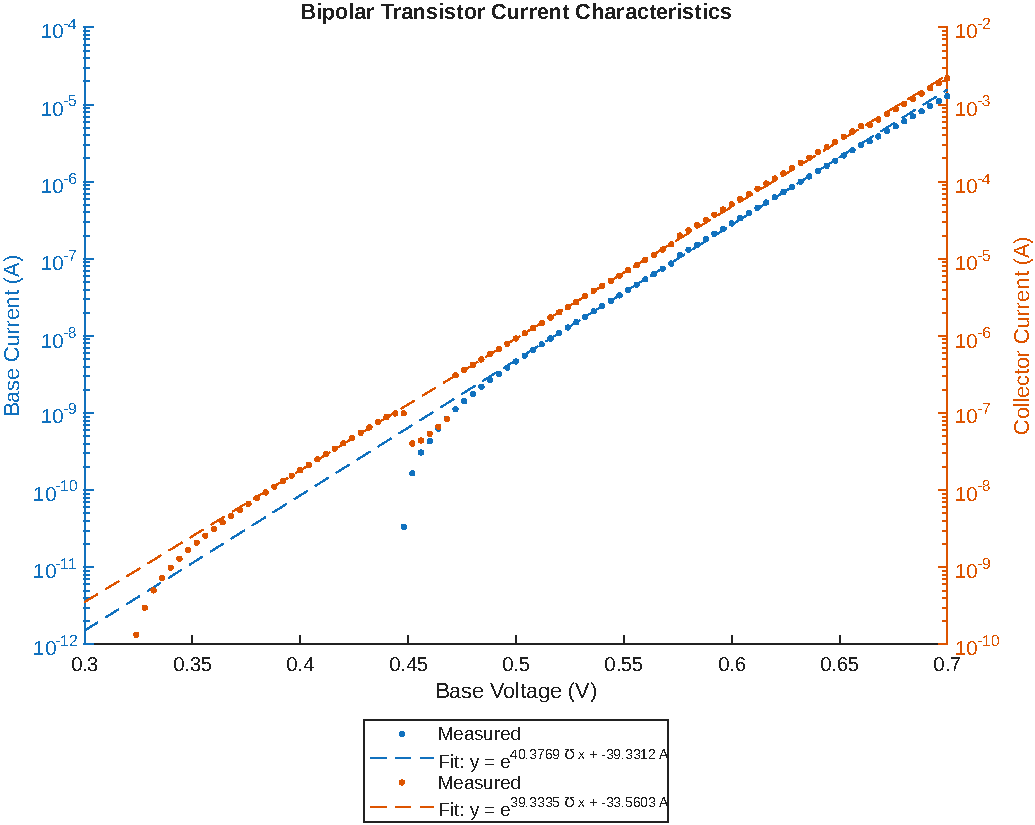
\includegraphics[width=0.7\linewidth]{../diagrams/lab3_exp1_BJT_Current_Characteristics.pdf}
		\caption{caption here}
		\label{fig:bjt_current_char}
	\end{figure}
	\begin{figure}[H]
		\centering
		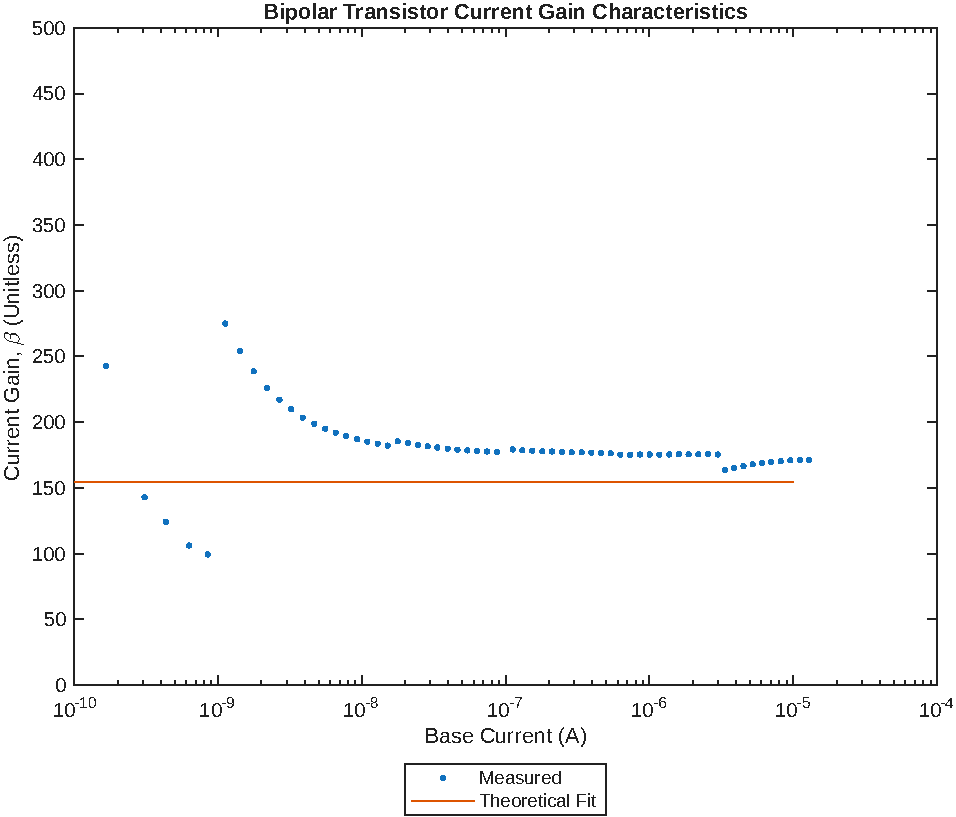
\includegraphics[width=0.7\linewidth]{../diagrams/lab3_exp1_BJT_Current_Gain_Characteristics.pdf}
		\caption{caption here}
		\label{fig:bjt_current_gain_char}
	\end{figure}
	\begin{figure}[H]
		\centering
		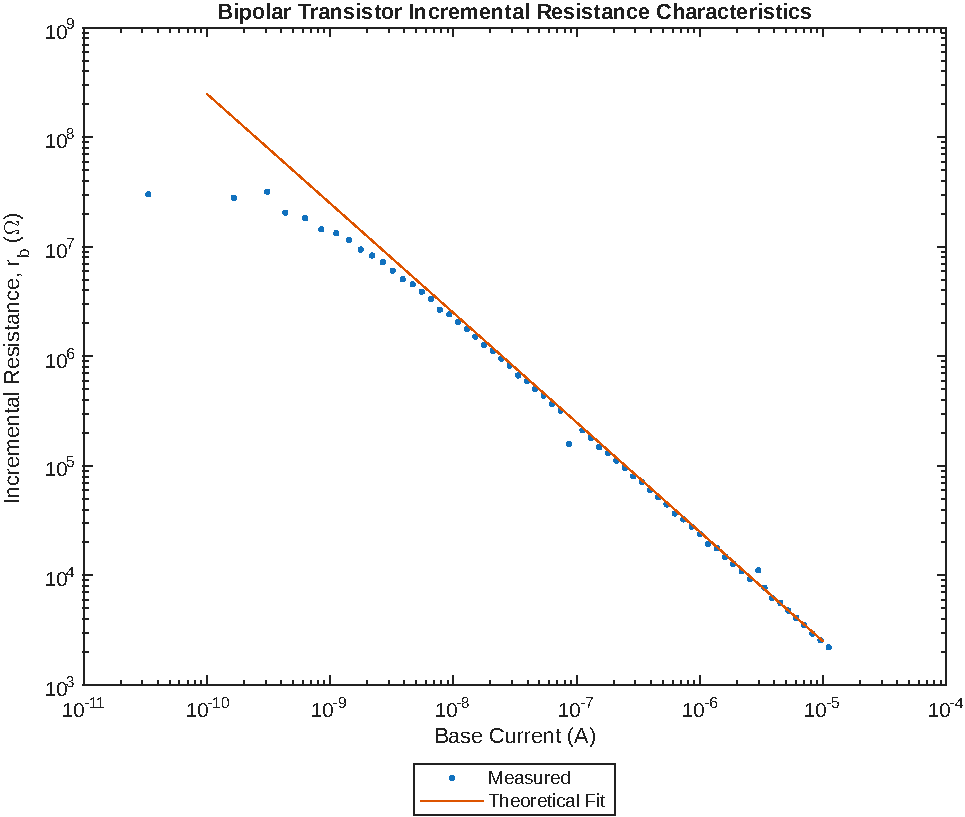
\includegraphics[width=0.7\linewidth]{../diagrams/lab3_exp1_BJT_Incremental_Resistance_Characteristics.pdf}
		\caption{caption here}
		\label{fig:bjt_incremental_resistance_char}
	\end{figure}
	\begin{figure}[H]
		\centering
		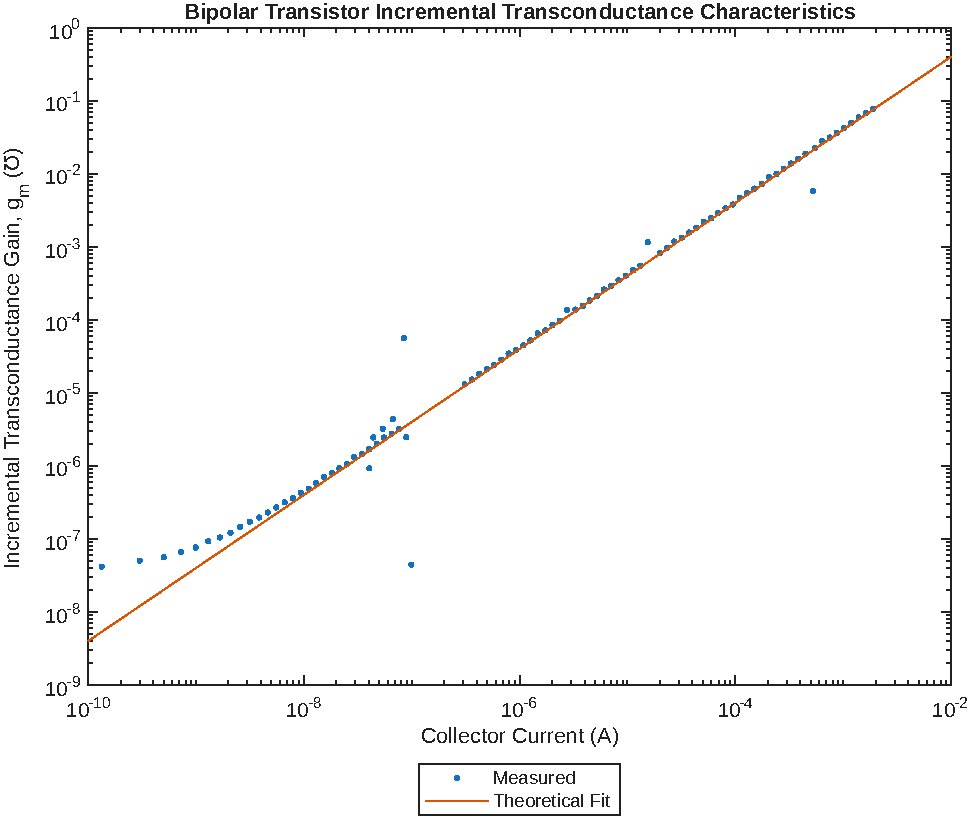
\includegraphics[width=0.7\linewidth]{../diagrams/lab3_exp1_BJT_Incremental_Transconductance_Characteristics.pdf}
		\caption{caption here}
		\label{fig:bjt_incremental_transconductance_char}
	\end{figure}
	\subsection{Analysis}
	\subsection{Discussion}
\section{Emitter-Degenerated Bipolar Characteristics}
	\subsection{Results}
	\begin{figure}[H]
 		\centering
   		\includegraphics[width=0.6\linewidth]{../diagrams/lab3_c2.pdf}
   		\caption{The schematic for the experimental setups used in Experiment 2. R values of 1k$\Omega$, 10k$\Omega$, and 100k$\Omega$ were used.}\label{fig:exp2_diag}
    \end{figure}
	\subsection{Analysis}
	\subsection{Discussion}
\section{Follower Voltage Transfer Characteristics}
	\subsection{Results}
	\begin{figure}[H]
 		\centering
   		\includegraphics[width=0.6\linewidth]{../diagrams/lab3_c3.pdf}
   		\caption{The schematic for the experimental setups used in Experiment 3. An R values of 1k$\Omega$ was used.}\label{fig:exp3_diag}
    \end{figure}
	After connecting the diode-connected transistor in the emitter-follower configuration as shown in \ref{fig:exp3_diag}., we measured the voltage transfer characteristic (VTC) of the circuit by sweeping the input voltage (Vin) and recording the corresponding output voltage (Vout). The VTC was plotted as Vout versus Vin, and a theoretical fit was also included for comparison. The plot is shown in Figure \ref{fig:exp3_plot1}.\\
    \begin{figure}[H]
        \centering
        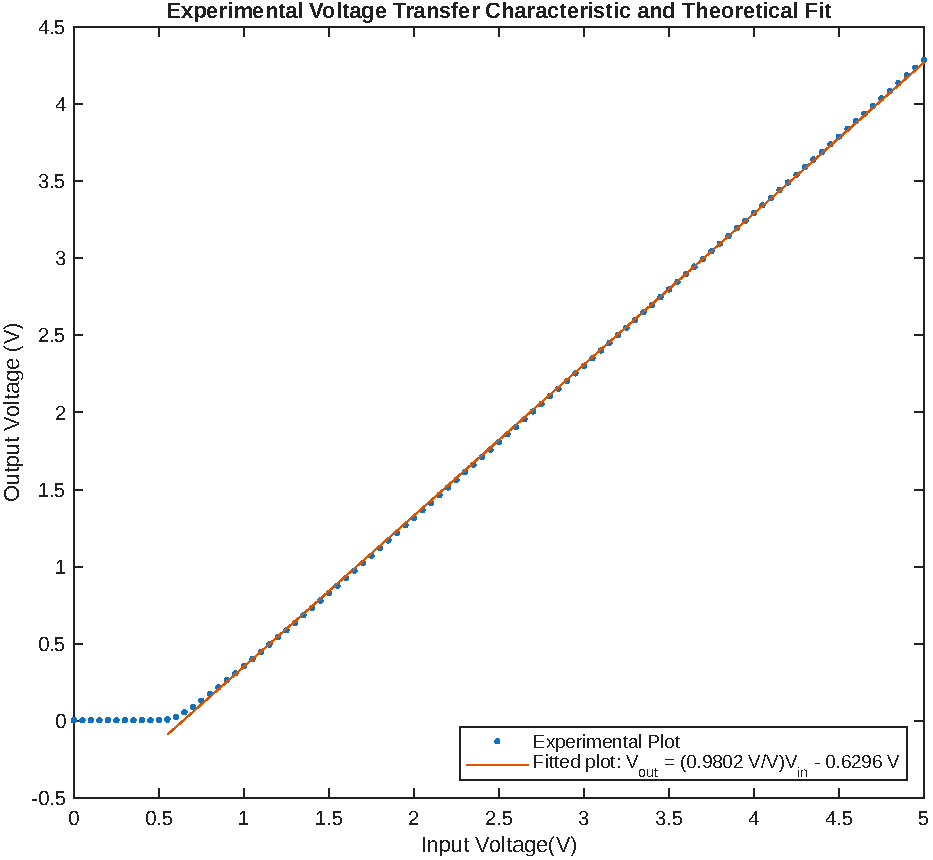
\includegraphics[width=0.7\linewidth]{../diagrams/lab3_exp3_plt1.pdf}
        \caption{plot showing the emitter-follower’s voltage transfer characteristic (VTC), which is a plot of Vout as a function of Vin, along with a theoretical fit. }\label{fig:exp3_plot1}
    \end{figure} 
	\subsection{Analysis}
	% What is the difference between Vin and Vout for this circuit? What determines this voltage difference?
	The difference between Vin and Vout remains close to constant as shown by the linear portion of the VTC. The average difference can be calculated to be 0.6799V. The difference between Vin and Vout in the emitter-follower configuration is determined by the base-emitter voltage of the diode connected transistor. This is determined by the current flowing through the transistor and the characteristics of the transistor itself. 
	
	\subsection{Discussion}
	% What is the incremental voltage gain of the emitter follower?
	The incremental voltage gain (Av) of the emitter follower can be calculated using the formula: Av = dVout/dVin. From the VTC plot, we can determine the slope of the curve at different points to find the incremental voltage gain which was 0.9802. The gain of the emitter follower is expected to be close to 1. However, due to the presence of the diode-connected transistor and the slight error in the smu, the actual gain is slightly less than 1.

\section{Inverter Voltage Transfer Characteristics}
	\subsection{Results}
	\begin{figure}[H]
 		\centering
   		\includegraphics[width=0.6\linewidth]{../diagrams/lab3_c4.pdf}
   		\caption{The schematic for the experimental setups used in Experiment 4. An R value of 1k$\Omega$, and mR values of 10k$\Omega$, 5k$\Omega$, and 2k$\Omega$ were used.}\label{fig:exp4_diag}
	\end{figure}
	\begin{figure}[H]
		\centering
		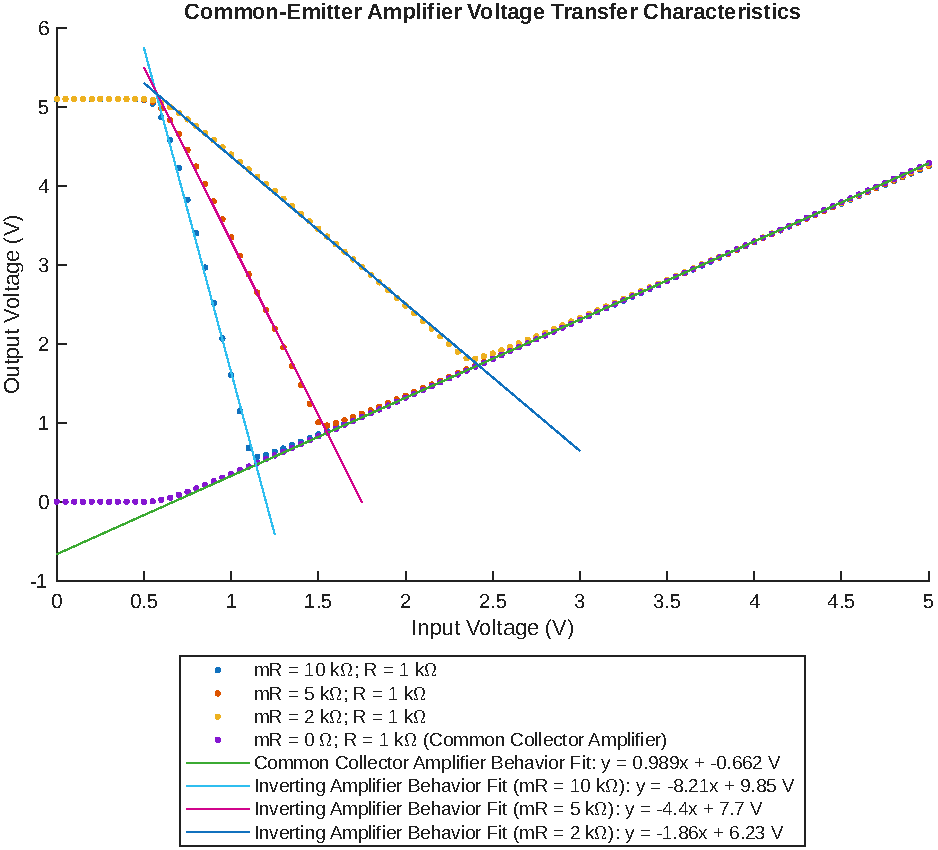
\includegraphics[width=0.7\linewidth]{../diagrams/lab3_exp4.pdf}
		\caption{caption here}
		\label{fig:thing}
	\end{figure}
	\subsection{Analysis}
	\subsection{Discussion}

%----------------------------------------------------------

\end{document}
